%!TEX root = Slic3r-Manual.tex

\subsection{\texttt{Skirt}} % (fold)
\label{sec:skirt}
\index{skirt}
\index{Print Settings!Skirt and brim!Skirt}

The \texttt{Skirt} setting adds an extrusion a short distance away from the perimiter of the object.  This can ensure that the material is flowing smoothly from the extruder before it starts on the model proper.

\begin{figure}[H]
\centering
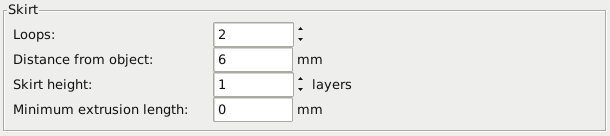
\includegraphics[keepaspectratio=true,width=1.0\textwidth]{expertmode/skirt_settings.png}
\caption{Skirt settings.}
\label{fig:skirt_settings}
\end{figure}

\begin{itemize}
    \index{Print Settings!Skirt and brim!Skirt!Loops}
    \item \texttt{Loops} - How many circuits should be completed before starting on the model.  One loop is usually sufficient.
    \index{Print Settings!Skirt and brim!Skirt!Distance from object}
    \item \texttt{Distance from object} - The millimeters between the object and the skirt.  The default of 6mm is usually sufficient.
    \index{Print Settings!Skirt and brim!Skirt!Skirt height}
    \item \texttt{Skirt height} - The number of layers to lay down a skirt for.  For ensuring the material is flowing smoothly, one layer is sufficient, however the skirt function can also be used to build walls around the object in case it should be protected from drafts.
    \index{Print Settings!Skirt and brim!Skirt!Minimum extrusion length}
    \item \texttt{Minimum extrusion length} - Dictates a minimum number of millimeters that the skirt should be, should the loop around the object not be enough.
\end{itemize}

% subsection skirt (end)
